% !TEX root = ../thesis.tex

\chapter{Einleitung und Motivation}

\paragraph{Ausblick:}
Dieses Kapitel dient zur allgemeinen Einführung in diese Masterarbeit. Dazu werden neben einer Einleitung und Motivation in das zugrundeliegende Thema, die grundlegenden Strukturen der Arbeit erläutert. Dazu gehören die Forschungsziele und Forschungsfragen, das verwendete Forschungsdesign, eine Übersicht der angedachten und tatsächlichen Zeitplanung sowie eine Erläuterung des Aufbaus der weiterführenden Teile dieser Arbeit.
\\
\hrule

Softwarefehler stellen einen erheblichen Auslöser für finanzielle Schäden und Rufschädigungen von Unternehmen dar. Solche Fehler reichen von kleineren \glqq Bugs\grqq{} bis hin zu schwerwiegenden Sicherheitslücken. Aus diesem Grund herrscht ein großes Interesse daran, einen Entwickler zu warnen, wenn er aktualisierten Softwarecode veröffentlicht, der möglicherweise einen Fehler beinhaltet. 

Zu diesem Zweck haben Forscher und Softwareentwickler im vergangenen Jahrzehnt verschiedene Techniken zur Fehlererkennung und Fehlervorhersage entwickelt, die zu einem Großteil auf Methoden und Techniken des \emph{Machine Learnings} basieren. Diese verwenden in der Regel historische Daten von fehlerhaften und fehlerfreien Änderungen an Softwaresystemen in Kombination mit einer sorgfältig zusammengestellten Menge von \emph{Attributen} (in der Regel Features genannt \footnote{Um einem missverständlichen und doppeldeutigen Gebrauch des Feature-Begriffes vorzubeugen, wird für die hier verwendete Beschreibung der Charakteristika von Daten auch im weiteren Verlauf dieser Ausarbeitung der Begriff \glqq Attribute\grqq{} verwendet.}), um einen gegebenen Klassifikator anzulernen beziehungsweise zu trainieren. Dieser dient dann dazu, ein akkurate Vorhersage zu treffen, ob eine neu erfolgte Änderung an einer Software fehlerbehaftet oder frei von Fehlern ist.

Die Auswahl an Lernverfahren für Klassifikatoren ist groß. Studien zeigen, aus diesem Pool von Verfahren sowohl Entscheidungsbaum-basierte (zum Beispiel J48, CART oder Random Forest) als auch bayessche Verfahren die meistgenutzten sind \cite{Son2019}. Alternative Lernmethoden sind Regression, k-Nearest-Neighbor oder künstliche neuronale Netze \cite{Challagulla2008}. Anzumerken ist allerdings, dass es keinen Konsens über die beste verfügbare Lernverfahren gibt, da jedes Verfahren unterschiedliche Stärken und Schwächen für bestimmte Anwendungsfälle aufweist.

Das Ziel dieser Arbeit ist die Entwicklung einer solchen Vorhersagetechnik für Softwarefehler basierend auf Software-Features. Diese beschreiben Inkremente der Funktionalität eines Softwaresystems. Die auf diese Weise entwickelten Softwaresysteme heißen Software-Produktlinien und bestehen aus einer Menge von ähnlichen Softwareprodukten. Sie zeichnen sich dadurch aus, dass sie eine gemeinsame Menge von Features sowie eine gemeinsame Codebasis besitzen \cite{Thuem2014}. Durch das Vorhandensein verschiedener Features entlang der Softwareprodukte, kann eine breite Variabilität innerhalb einer Produktlinie erreicht werden. 

\textbf{ÜBERARBEITEN!}

Die nachfolgende Abbildung 1.1 zeigt den zentralen Prozess der Entwicklung einer Produktlinie. Aufgeteilt wird dieser in das Domain Engineering und das Application Engineering. Im Rahmen des Domain Engineerings wird ein sogenanntes Variabilitätsmodell (Variability Model) erzeugt, welches durch die Kombination der wählbaren Features beschrieben wird \cite{Apel2013}. Gängige Implementationstechniken für Features reichen von einfachen Lösungen durch Annotationen basierend auf Laufzeitparametern oder Präprozessor-Anweisungen bis hin zu verfeinerten Lösungen basierend auf erweiterten Programmiermethoden, wie zum Beispiel Aspektorientierung. In Teilen dieser Implementierungstechniken wird jedes Feature wird als wiederverwendbares Domain Artifact modelliert und gekapselt, welches im Prozess des Application Engineerings in Form einer Konfiguration zusammen mit weiteren Features, im Hinblick auf die gewünschte Funktionalität der Software, ausgewählt werden kann. Ein Software Generator erzeugt dann die gewünschten Software Produkte basierend auf den bereits zuvor genannten Implementationstechniken für Features.

\begin{figure}[H]
    \centering
    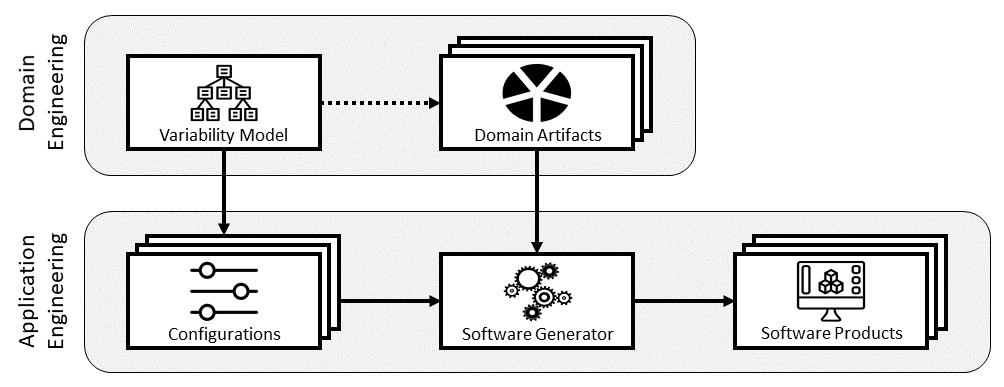
\includegraphics[width=\textwidth]{images/SPL}
    \caption{Generierung von Software-Produktlinien nach \cite{Thuem2014}\label{fig:spl}}
\end{figure}
 
Das Ziel dieser Arbeit ist die Entwicklung einer auf Machine Learning gestützten Vorhersagetechnik für defekte Software-Features. Dieser bisher in wissenschaftlichen Papern nur einmal betrachtete Ansatz ist aufgrund mehrerer Gründe chancenreich:

\begin{enumerate}
\item Wenn ein bestimmtes Feature in der Vergangenheit mehr oder weniger fehleranfällig war, so ist eine Änderung, die das Feature aktualisiert, wahrscheinlich ebenfalls mehr oder weniger fehleranfällig. 
\item Features, die mehr oder weniger fehleranfällig scheinen, könnten besondere Eigenschaften haben, die im Rahmen der Fehlervorhersage verwendet werden können.
\item Code, der viel Feature-spezifischen Code enthält (insbesondere die sogenannten Feature-Interaktionen), ist möglicherweise fehleranfälliger als sonstiger Code.
\end{enumerate}

Das zuvor genannte Ziel der Arbeit setzt sich aus mehreren Teilzielen zusammen. Dazu zählen die Erstellung eines Datensets zum Trainieren von Machine-Learning-Klassifikatoren sowie das Anlernen einer repräsentativen Auswahl an Klassifikatoren mit anschließender vergleichender Evaluation dieser. Ein genauer Überblick über die Forschungsziele befindet sich im \hyperref[research_objectives]{nächsten Unterkapitel}.

Sollte sich im Rahmen der Evaluation einer dieser Klassifikatoren als besonders effektiv erweisen, so würde diese Arbeit den Stand der Technik hinsichtlich der Fehlererkennung in Features vorantreiben und Organisationen erlauben, bessere Einblicke in die Fehleranfälligkeit von Änderungen in ihrer Codebasis zu erhalten.

\section{Forschungsziele und Forschungsfragen}

\textbf{ÜBERARBEITEN!}

Wie bereits in der Einleitung beschrieben, ist das übergeordnete Ziel dieser Arbeit die Entwicklung einer Vorhersagetechnik für Fehler in featurebasierter Software unter Zuhilfenahme von Methoden des Machine Learnings. Dazu ist vorgesehen, das Augenmerk auf Commits von Versionierungssystemen, wie beispielsweise Subversion oder Git, zu richten. Ein Commit bezeichnet dabei die zur Verfügungstellung einer aktualisierten Version einer Software. Als Datenbasis für das Trainieren der Klassifikatoren dienen dann fehlerhafte und fehlerfreie Commits von featurebasierter Software. Dies ermöglicht es, ausstehende defekte Commits vorherzusagen und das Risiko der Konsequenzen von Softwarefehlern zu senken.

Der Prozess der Entwicklung der Vorhersagetechnik ist in drei zu erreichende Forschungsziele eingeteilt. Jedem Forschungsziel werden Forschungsfragen zugeordnet, deren Aufklärung einen zusätzlichen Teil zur Erfüllung der Ziele beiträgt. Im Folgenden werden die Forschungsziele (RO – „research objective“) mit ihren zugehörigen Forschungsfragen (RQ – „research question“) vorgestellt.

\label{research_objectives}
\begin{flushleft}
\textsc{RO1: Erstellung eines Datensets zum Trainieren von relevanten Machine-
Learning-Klassifikatoren}\medskip\linebreak 
\emph{RQ1a: Welche Daten kommen für die Erstellung des Datensets in Frage?}\linebreak
\emph{RQ1b: Wie weit müssen die Daten vorverarbeitet werden, um sie für das Training nutzbar zu machen?}

\textsc{RO2: Identifikation und Training einer Auswahl von relevanten Machine Learning Klassifikatoren basierend auf dem Datenset}\medskip\linebreak 
\emph{RQ2: Welche Machine Learning Klassifikatoren kommen für die gegebene Aufgabe in Frage?}

\textsc{RO3: Evaluierung und Gegenüberstellung der Klassifikatoren sowie Vergleich zu modernen Vorhersagetechniken, die keine Features nutzen}\medskip\linebreak 
\emph{RQ3a: Welche miteinander vergleichbaren Merkmale besitzen die Klassifikatoren?}\linebreak 
\emph{RQ3b: Welche Metriken können für den Vergleich verwendet werden?}\linebreak 
\emph{RQ3c: Welche Vor- und Nachteile besitzt ein Klassifikator?}\linebreak 
\emph{RQ3d: Wie lassen sich die Klassifikatoren mit weiteren Vorhersagetechniken, die keine Features nutzen, vergleichen?}
\end{flushleft}

\label{phases_definition}

Zusätzlich zu den drei genannten Forschungszielen umfasst die Bearbeitung der Masterarbeit eine Vor- und Nachbereitung, sodass sich insgesamt fünf Arbeitsphasen ergeben. Diese werden in den weiteren Unterkapiteln näher erläutert. Als finale Vorhersagetechnik wird jener Klassifikator verwendet, der sich im Rahmen der Gegenüberstellung im Verlauf der Evaluation als am effektivsten erweist.

\section{Forschungsdesign}

Die für diese Arbeit gewählte Methodik basiert auf dem Prozessmodell Cross-Industry Standard Process for Data Mining, kurz CRISP-DM, nach \cite{Chapman2000}. Es wird als Vorlage für die Arbeitsphasen zur Erreichung der Forschungsziele dieser Arbeit verwendet. 
Da der überwiegende praktische Teil dieser Arbeit auf Programmierung im Bereich des Machine Learning konzentriert, bildet das CRISP-DM Prozessmodell ein passendes vordefiniertes Vorgehen. Die nachfolgende \autoref{fig:crisp1} zeigt eine grafische Aufarbeitung des Prozessmodells mit seinen sechs zugehörigen Phasen sowie den Verbindungen zwischen diesen.

\begin{figure}[H]
    \centering
    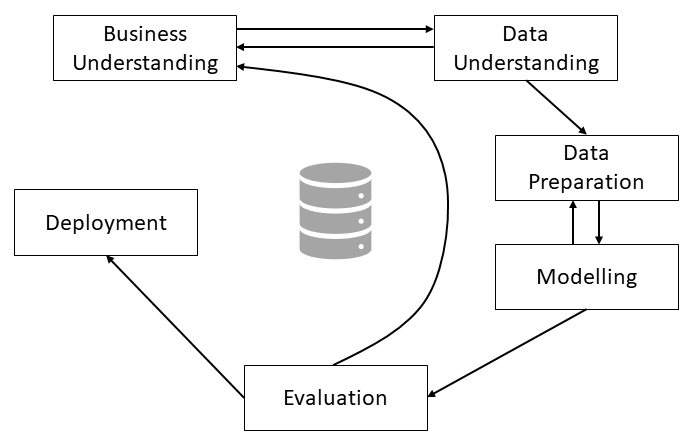
\includegraphics[width=\textwidth]{images/CRISP-DM1}
    \caption{CRISP-DM Prozessmodells nach \cite{Chapman2000}}\label{fig:crisp1}
\end{figure}

Das CRISP-DM Prozessmodell würde ursprünglich, wie der Name bereits andeutet, für die Erarbeitung von Data Mining Projekten entwickelt, eignet sich jedoch auch zur Verwendung im Rahmen eines Machine Learning Projektes, da sich die in beiden Bereichen verwendeten Methoden und Prozesse zu einem erheblichen Teil überlagern. Ein Überblick über die sechs Phasen des Prozessmodells ist in \autoref{fig:crisp} dargestellt. Zusätzlich umfasst diese Abbildung die Zuordnung der Arbeitsphasen, die im \hyperref[phases_definition]{vorherigen Unterkapitel} definiert wurden. Eine Erläuterung der Phasen des Prozessmodells erfolgt im Anschluss der Abbildung. Einen genauen Überblick über den konkreten Umfang der Arbeitsphasen, aufgeteilt in jeweilige Unterziele und zu erfüllende Aufgaben, bietet das im Anschluss \hyperref[timecourse] {folgende Unterkapitel}. 

\begin{figure}[H]
    \centering
    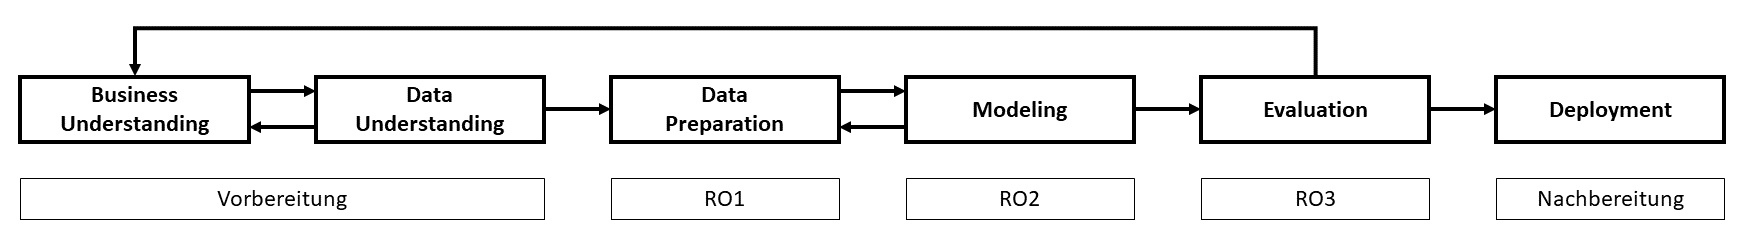
\includegraphics[width=\textwidth]{images/CRISP-DM}
    \caption{Phasen des CRISP-DM Prozessmodells nach \cite{Chapman2000} mit Zuordnung der Arbeitsphasen}\label{fig:crisp}
\end{figure}

Die ersten beiden Phasen \emph{Business Understanding} und \emph{Data Understanding} widmen sich der Vorbereitung der Arbeit. Die initiale Phase umfasst dabei die allgemeine Einarbeitung in das zugrundeliegende Thema und der Formulierung der Forschungsziele. Anzumerken ist, dass diese Phase bereits vor der sechsmonatigen Bearbeitungszeit der Arbeit beginnt und somit schon das Verfassen dieses Proposals als Teilaufgabe dieser Phase gezählt werden kann, da es auch eine grobe Einarbeitung in das Thema erfordert.

Die darauffolgende Phase \emph{Data Understanding} dient der Suche und Einsicht von für den weiteren Verlauf der Phasen relevanten Daten und, falls vorhanden, vorgefertigten Datensets. Da Commits als Datenbasis zur Erlernung der Klassifikatoren betrachtet werden, wird der überwiegende Teil der Suche nach Daten auf dem Onlinedienst GitHub stattfinden, welchem das Versionierungssystemen Git zugrunde liegt. Für die weiteren Phasen ist es von besonderer Bedeutung, den Aufbau der Daten sorgfältig zu untersuchen.

Die dritte Phase \emph{Data Preparation} kümmert sich um die Erstellung eines endgültigen Datensets und den dort hinführenden Prozessen. Diese Phase ist deckungsgleich mit den Anforderungen des ersten Forschungsziels.

Zur Anwendung kommt das im vorherigen Schritt erstellte Datenset in der Phase \emph{Modeling}. In dieser werden die Data-Mining-Algorithmen und -Techniken gemäß den zugrundeliegenden Anforderungen auf das Datenset angewendet. Adaptiert an das Lernen der Machine Learning Klassifikatoren spiegelt dies die Arbeitsphase zur Erfüllung des zweiten Forschungsziels dar. 

Die fünfte Phase umfasst die \emph{Evaluation} der Resultate des zuvor erfolgten Schrittes und deckt somit die Erfüllung des dritten Forschungsziels ab.

Die Nachbereitung der Arbeit wird durch die Phase \emph{Deployment} abgedeckt. Diese umfasst die Erstellung der finalen Ausarbeitung sowie der Abschlusspräsentation und der anschließenden Vorführung dieser im Rahmen des Kolloquiums.

Es ist zu erkennen, dass die Beschreibung der Arbeitsphasen weitestgehend auf einem theoretischen Level verfasst wurde. Es wird anhand der fünf CRISP-DM-Phasen gezeigt, was für den erfolgreichen Abschluss der Arbeit absolviert werden muss. Die Erörterung der Frage, wie die einzelnen zu erledigenden Aufgaben durchgeführt werden müssen, ist Teil der Vorbereitung der Arbeit. Im Rahmen der Phasen Business Understanding und Data Understanding wird nach einer eingehenden Recherche die genaue Arbeitsplanung festgelegt (siehe Unterziele der ersten Phase im \hyperref[timecourse] {folgenden Unterkapitel}).  

\section{Zeitplanung}
\label{timecourse}

\textbf{ANPASSEN AN TATSÄCHLICHEN ABLAUF}

Im Nachfolgenden wird die vorläufige Ablaufplanung der Arbeit aufgezeigt. Die Ordnung erfolgt gemäß der Aufteilung in die fünf zuvor beschriebenen Arbeitsphasen. Die geschätzte Dauer der verschiedenen Unterziele wird jeweils in Tagen, Wochen oder Monaten angegeben. Zur Verfügung stehen insgesamt sechs Monate Bearbeitungszeit.

\underline{Phase 1: Vorbereitung}
\begin{table}[H]
\refstepcounter{table}
\label{tab:phase1}
\resizebox{\linewidth}{!}{%
\begin{tabular}{|l|c|c|l} 
\cline{1-3}
\textbf{Unterziele}                                                                                                                                                                                                                                                                                                                               & \begin{tabular}[c]{@{}c@{}}\textbf{geplante}\\\textbf{Dauer} \end{tabular} & \begin{tabular}[c]{@{}c@{}}\textbf{tatsächliche}\\\textbf{Dauer}\end{tabular} &                                              \\ 
\hline
\begin{tabular}[c]{@{}l@{}}Strukturierte Literaturrecherche\\ - Techniken der featurebasierten Softwareprogrammierung\\ - Techniken zur Fehlererkennung in Software\\ - Klassifikation mittels Machine Learning\\ - Klassifikationsmethoden\\ - Auswahl der Programmiersprache\\ - Tool- und Libraryauswahl\\ - Evaluationsmetriken \end{tabular} & 2 Wochen                                                                   & TBD                                                                           & \multicolumn{1}{l|}{Business Understanding}  \\ 
\hline
\begin{tabular}[c]{@{}l@{}}Recherche zur Bildung eines Datensets\\ - Merkmale / Aufbau eines Datensets\\ - Suche nach Datenquellen\\ - Suche nach vorgefertigten Datensets\\ - Prüfung der Daten / Datensets auf Eignung\\ - Analyse des Aufbaus der Daten / der Datensets \end{tabular}                                                          & 1 Woche                                                                    & TBD                                                                           & \multicolumn{1}{l|}{Data Understanding}      \\ 
\hline
\multicolumn{1}{r|}{Total:}                                                                                                                                                                                                                                                                                                                       & 3 Wochen                                                                   & TBD                                                                           &                                              \\
\cline{2-3}
\end{tabular}
}
\end{table}

\underline{Phase 2: Forschungsziel 1 – Erstellung des Datensets (Data Preparation)}
\begin{table}[H]
\refstepcounter{table}
\label{tab:phase2}
\resizebox{\linewidth}{!}{%
\begin{tabular}{|l|c|c|} 
\hline
\textbf{Unterziele}                                                                                                                                                                                                            & \textbf{geplante Dauer}  & \textbf{tatsächliche Dauer}  \\ 
\hline
\begin{tabular}[c]{@{}l@{}}finale Datenauswahl\\ - Festlegung von Kriterien \end{tabular}                                                                                                                                      & 1 Woche                  & TBD                          \\ 
\hline
\begin{tabular}[c]{@{}l@{}}Datenbereinigung\\ - "Preprocessing" \end{tabular}                                                                                                                                                  & 1 Woche                  & TBD                          \\ 
\hline
\begin{tabular}[c]{@{}l@{}}finale Konstruktion des Datensets\\ - Integration der Daten und des Feature-Aspekts\\ - erneute abschließende Bereinigung sowie Formatierung\\ - Teilung in Training-Set und Test-Set \end{tabular} & 1 Woche                  & TBD                          \\ 
\hline
\multicolumn{1}{r|}{Total:}                                                                                                                                                                                                    & 3 Wochen                 & TBD                          \\
\cline{2-3}
\end{tabular}
}
\end{table}

\underline{Phase 3: Forschungsziel 2 – Training der Machine Learning Klassifikatoren (Modeling)}
\begin{table}[H]
\refstepcounter{table}
\label{tab:phase3}
\begin{tabular}{|l|c|c|} 
\hline
\textbf{Unterziele}                & \textbf{geplante Dauer}  & \textbf{tatsächliche Dauer}  \\ 
\hline
Auswahl geeigneter Klassifikatoren & 1 Woche                  & TBD                          \\ 
\hline
Training der Klassifikatoren       & 3 Wochen                 & TBD                          \\ 
\hline
\multicolumn{1}{r|}{Total:}        & 4 Wochen                 & TBD                          \\
\cline{2-3}
\end{tabular}
\end{table}

\underline{Phase 4: Forschungsziel 3 – Evaluation und Vergleich der Machine Learning Klassifikatoren}
\begin{table}[H]
\refstepcounter{table}
\label{tab:phase4}
\resizebox{\linewidth}{!}{%
\begin{tabular}{|l|c|c|} 
\hline
\textbf{Unterziele}                                                                                                                                                                       & \textbf{geplante Dauer}  & \textbf{tatsächliche Dauer}  \\ 
\hline
\begin{tabular}[c]{@{}l@{}}Evaluation der einzelnen Klassifikatoren\\ - Festlegung der Bewertungsmetriken\\ - Anwendung des Test-Sets\\ - Berechnung der Bewertungsmetriken \end{tabular} & 2 Wochen                 & TBD                          \\ 
\hline
Vergleich der Klassifikatoren anhand der Metriken                                                                                                                                         & 2 Wochen                 & TBD                          \\ 
\hline
Vergleich mit weiteren Vorhersagetechniken, die nicht auf Features setzen                                                                                                                 & 1 Woche                  & TBD                          \\ 
\hline
\multicolumn{1}{r|}{Total:}                                                                                                                                                               & 5 Wochen                 & TBD                          \\
\cline{2-3}
\end{tabular}
}
\end{table}

\underline{Phase 5: Nachbereitung (Deployment}
\begin{table}[H]
\refstepcounter{table}
\label{tab:phase5}
\resizebox{\linewidth}{!}{%
\begin{tabular}{|l|c|c|} 
\hline
\textbf{Unterziele}                                                                                                                          & \textbf{geplante Dauer}  & \textbf{tatsächliche Dauer}  \\ 
\hline
\begin{tabular}[c]{@{}l@{}}Besprechung der vorangegangenen Arbeit mit Betreuer\\ - Umsetzung möglicher Verbesserungsvorschläge \end{tabular} & 1 Woche                  & TBD                          \\ 
\hline
Erstellung der Ausarbeitung                                                                                                                  & 7 Wochen                 & TBD                          \\ 
\hline
Erstellung der Abschlusspräsentation                                                                                                         & 1 Woche                  & TBD                          \\ 
\hline
\multicolumn{1}{r|}{Total:}                                                                                                                  & 9 Wochen                 & TBD                          \\
\cline{2-3}
\end{tabular}
}
\end{table}

* Die Erstellung der Ausarbeitung ist ein laufender Prozess über den gesamten Verlauf der Bearbeitungszeit. Der hier erwähnte siebenwöchige Zeitraum dient unter Anderem zur Korrektur beziehungsweise Verbesserung hinsichtlich des Feedbacks des Betreuers und zur abschließenden Finalisierung.

Die nachfolgende Abbildung zeigt den zeitlichen Ablauf der Arbeit als Gantt-Chart inklusive konkreter Datumsangaben. Eine größere Version des Plans befindet sich im Anhang.

\begin{figure}[H]
    \centering
    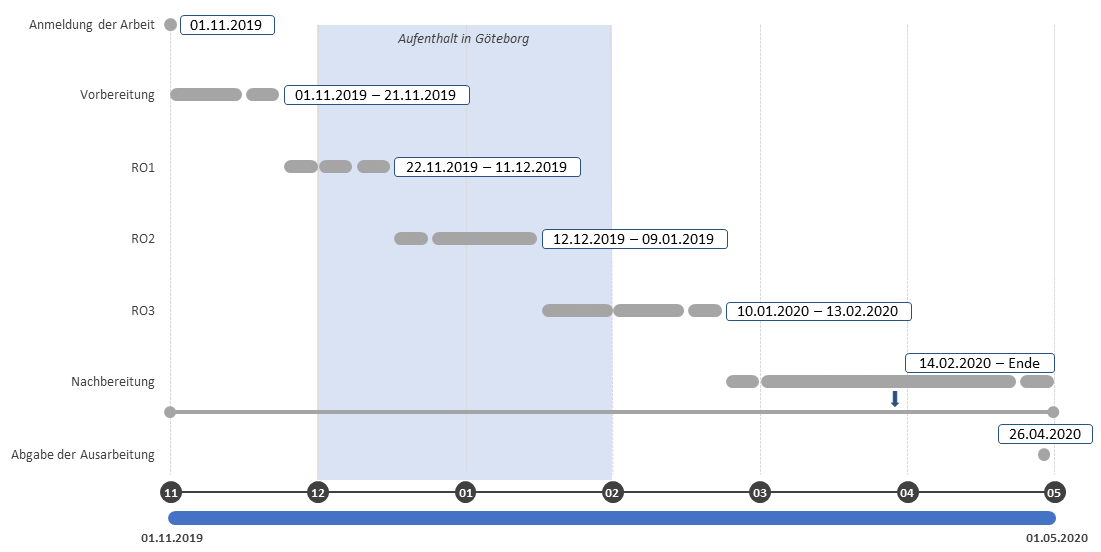
\includegraphics[width=\textwidth]{images/Zeit}
    \caption{Zeitlicher Ablaufplan der Arbeit als Gantt-Chart}\label{fig:zeit}
\end{figure}

\section{Aufbau der Arbeit}

Diese Ausarbeitung ist in sechs Kapitel unterteilt. Das erste Kapitel, welches mit diesem Abschnitt abgeschlossen wird, diente zur Einführung in das Thema der Masterarbeit. Ebenso stellte es die theoretischen Rahmenbedingungen der Arbeit vor. Das zweite Kapitel \glqq Hintergrund\grqq{} dient zur Vermittlung von Basiswissen zu den grundlegenden Themenkomplexen dieser Ausarbeitung. Dazu wird zunächst die featurebasierte Softwareentwicklung vorgestellt, ehe dann die Machine-Learning-Klassifikation sowie die darauf aufbauende Fehlervorhersage erläutert werden. Die zwei darauffolgenden Kapitel widmen sich der Auseinandersetzung des praktischen Teils dieser Masterarbeit in Form der Erstellung des featurebasierten Datensets sowie des Trainings der Machine-Learning-Klassifikatoren. Die Gegenüberstellung und Evaluation dieser Klassifikatoren erfolgt im fünften Kapitel inklusive eines Vergleiches zu nicht-featurebasierten Methoden zur Fehlererkennung. Eine abschließende Zusammenfassung sowie ein Ausblick auf weiterführende Projekte, die auf diese Masterarbeit aufbauen können, erfolgen im abschließenden sechsten Kapitel.

Zusätzlich wird die Ausarbeitung von zahlreichen Abbildungen zur verständlicheren Verdeutlichung von Zusammenhängen ergänzt.

\cleardoublepage
